\documentclass[11pt]{article}
\usepackage[margin=1in]{geometry}
\usepackage{graphicx}
\usepackage{booktabs}
\usepackage{array}
\usepackage{longtable}
\usepackage{hyperref}
\usepackage{float}

\setlength{\parindent}{0pt}
\setlength{\parskip}{0.6em}

\title{Progress Report 1\\\textbf{Detecting and Mitigating Simple IoT-Based DoS Attacks}}
\author{Group 8}
\date{}

\begin{document}
\maketitle

\section*{Overview}
Internet of Things (IoT) devices are now widely used in homes, campuses, and enterprise environments, but many of them still operate with limited built-in security protections. Because of this, compromised IoT devices are often used to launch denial-of-service (DoS) attacks that can disrupt service availability. The purpose of this project is to design and evaluate a lightweight and explainable system for detecting simple IoT-based DoS attacks using simulated traffic traces and threshold-based analysis.


\section*{Objectives}
The main goal of the project is to determine whether simple traffic-based metrics can distinguish normal IoT behavior from attack traffic. In particular, the system is designed to analyze packet traces over short time windows, detect suspicious deviations from baseline behavior, and simulate a mitigation response once an attack is identified.

To make the study more realistic without making it overly complex, the implementation includes not only normal traffic and attack traffic, but also a benign burst phase that represents legitimate but sudden increases in communication, such as a firmware update. This allows the project to examine both detection capability and false positive behavior.

\section*{System Design and Implementation}
The overall pipeline follows the original project plan closely: traffic generation, feature extraction, detection, and mitigation, with evaluation and visualization added on top. The current codebase is organized into modular scripts, each responsible for one part of the pipeline. Table~\ref{tab:modules} summarizes the structure of the implementation.

\begin{table}[H]
\centering
\caption{Project scripts and their responsibilities}
\label{tab:modules}
\begin{tabular}{>{\raggedright\arraybackslash}p{4.2cm} >{\raggedright\arraybackslash}p{10cm}}
\toprule
\textbf{Script} & \textbf{Responsibility} \\
\midrule
\texttt{traffic\_generator.py} & Generates synthetic IoT traffic and writes a single PCAP containing four phases: normal traffic, benign burst traffic, UDP flood traffic, and TCP SYN flood traffic. It also creates \texttt{labels.csv} with per-second ground-truth labels. \\
\texttt{feature\_extractor.py} & Reads the generated PCAP and computes per-second features, including packets per second, bytes per second, SYN packets per second, number of unique destination ports, and number of unique destination IPs. \\
\texttt{detector.py} & Implements the adaptive threshold detector. For each time window, it computes a rolling baseline mean and standard deviation and flags the window as suspicious if any selected feature exceeds its threshold. \\
\texttt{mitigation.py} & Simulates mitigation by recording a log entry for windows predicted as attack, such as dropping or rate-limiting the suspicious traffic source. \\
\texttt{evaluator.py} & Computes performance metrics including accuracy, precision, recall, false positive rate, and F1 score. It also performs a threshold sweep to show tradeoffs across different settings. \\
\texttt{visualizer.py} & Produces the main figures used in analysis, including a time-series plot of feature values with ground-truth labels and a threshold sweep plot. \\
\texttt{main.py} & Orchestrates the entire workflow: optional traffic generation, feature extraction, detection, mitigation simulation, evaluation, and plot generation. It also handles command-line arguments. \\
\bottomrule
\end{tabular}
\end{table}

\section*{Methodology}
The system uses a synthetic traffic model with four sequential phases. The first phase represents normal IoT communication, which provides a baseline for expected behavior. The second phase introduces a benign burst to imitate a legitimate temporary spike in activity. The third and fourth phases simulate two DoS attack types: a UDP flood and a TCP SYN flood. Ground-truth labels are assigned on a per-second basis so that each time window can later be compared against the detector's prediction.

After traffic generation, packets are aggregated into one-second windows and transformed into a set of lightweight traffic features. These features include packet rate, byte rate, SYN rate, destination-port diversity, and destination-IP diversity. The detector then analyzes these features using a rolling baseline. For each feature, the recent baseline mean and standard deviation are estimated, and a window is flagged if the observed value exceeds the configured threshold multiplier.

Mitigation is currently simulated rather than enforced through firewall rules. This decision keeps the project easier to run in a course environment while still allowing the report to study how detection results could trigger a defensive response. Finally, the system evaluates its predictions using classification metrics and produces visualizations to illustrate feature behavior and threshold tradeoffs.

\section*{Project Progress}
At this stage, the full offline pipeline has been implemented and tested on synthetic traces. The project has moved beyond initial planning and now includes an end-to-end workflow that can generate traffic, compute features, detect suspicious activity, log mitigation decisions, and summarize results through metrics and figures.

A key improvement over the original baseline idea is the inclusion of adaptive thresholds rather than only fixed thresholds. This allows the detector to respond to changing traffic conditions in a more flexible way. In addition, the implementation now includes two attack types instead of one, along with benign burst traffic to test the system's susceptibility to false positives. These additions make the project more rigorous while keeping it within manageable scope.

\section*{Preliminary Results}
Initial experiments on synthetic traces show that the detector can separate clearly malicious flood traffic from baseline traffic in some settings, but the current performance also indicates that the detector still misses a significant portion of attack windows. This is especially visible in the recall value, which remains low in the latest run. At the same time, the false positive rate is relatively modest, suggesting that the current threshold configuration is conservative.

These results are useful even though they are not yet strong. They show that the overall framework is working, but the detector still needs additional threshold tuning and possibly feature refinement in order to improve attack coverage without sharply increasing false alarms. Table~\ref{tab:metrics} summarizes the latest metrics.

\begin{table}[H]
\centering
\caption{Metrics from the latest experimental run}
\label{tab:metrics}
\begin{tabular}{lc}
\toprule
\textbf{Metric} & \textbf{Value} \\
\midrule
Accuracy & 0.7273 \\
Precision & 0.4167 \\
Recall & 0.1250 \\
False Positive Rate & 0.0614 \\
F1 Score & 0.1923 \\
\bottomrule
\end{tabular}
\end{table}

\begin{figure}[H]
  \centering
  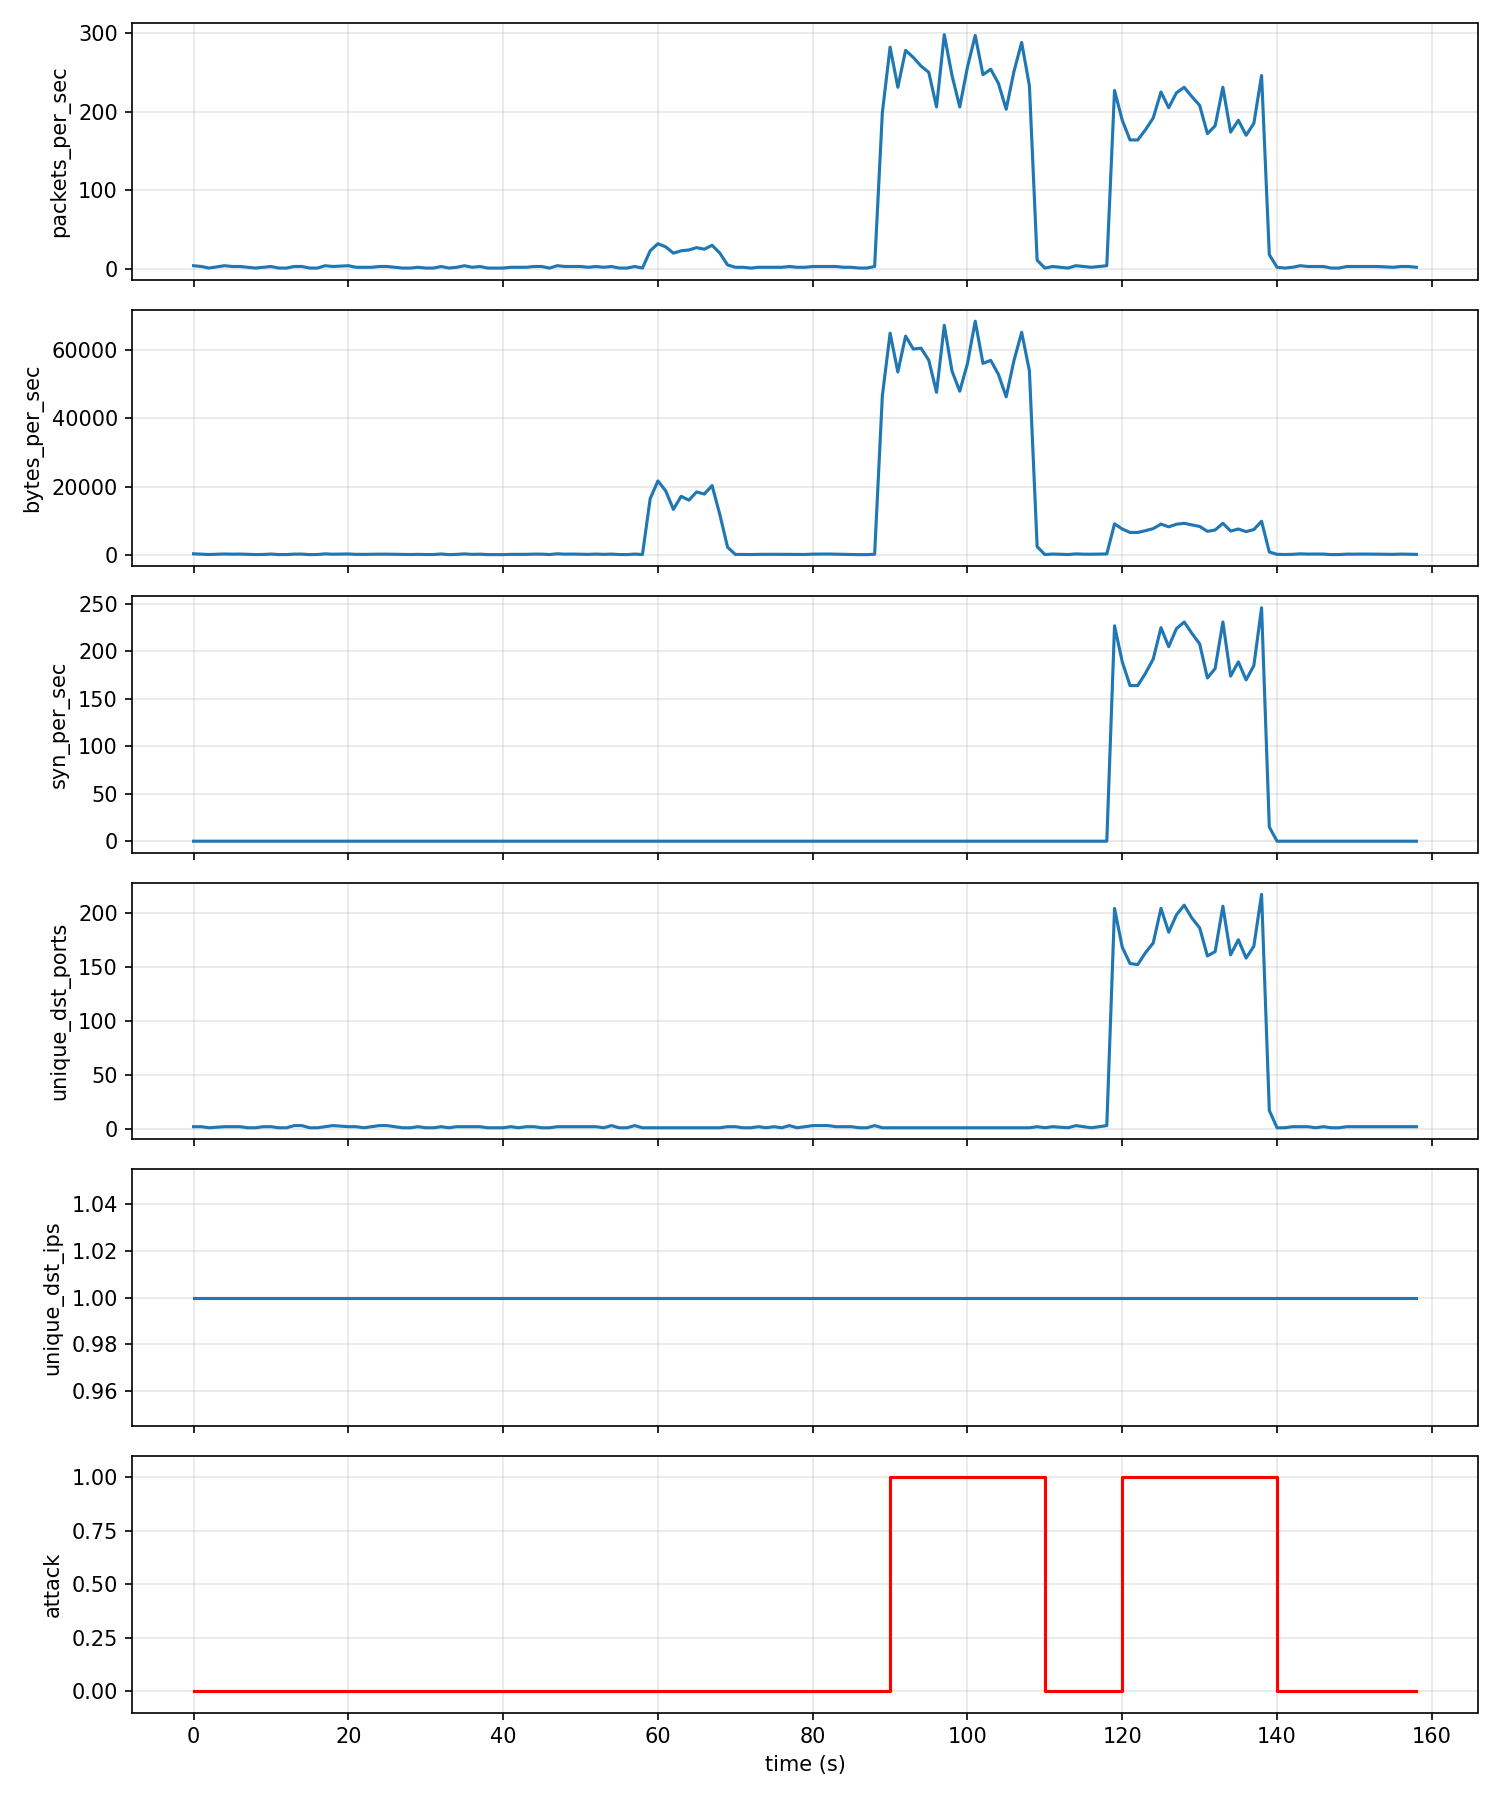
\includegraphics[width=0.95\linewidth]{figures/timeseries.png}
  \caption{Per-second traffic features over time with ground-truth labels for normal and attack periods.}
\end{figure}

\begin{figure}[H]
  \centering
  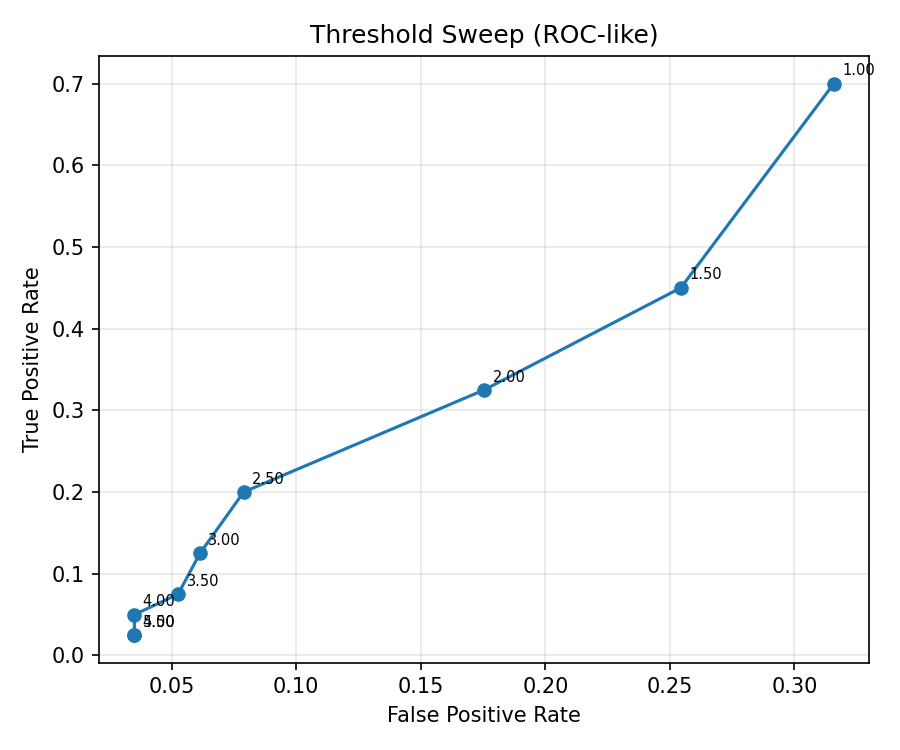
\includegraphics[width=0.72\linewidth]{figures/roc_like.png}
  \caption{Threshold sweep showing the tradeoff between attack detection sensitivity and false positives under different settings.}
\end{figure}

\section*{Challenges and Current Limitations}
Several challenges have become clear during the implementation process. First, because the dataset is synthetic, it does not fully capture the variety and unpredictability of real IoT traffic. Second, the inclusion of benign burst traffic shows that legitimate spikes can resemble malicious behavior, which makes threshold selection more difficult. Third, the simulated attack phases are cleanly separated in time, whereas real traffic would likely contain more noise and overlap.

Another important limitation is that the current mitigation stage is only simulated. This is acceptable for the scope of the course project, but it means the work should be interpreted as a prototype for detection and response logic rather than a deployed defense system.

\section*{Plan for the Remaining Work}
The next phase of the project will focus on improving both the performance of the current detector and the overall quality of the evaluation. The first priority is to run additional experiments under multiple random seeds and parameter settings so that the reported results are more robust. The project will also include a direct comparison between fixed-threshold detection and adaptive-threshold detection in order to better understand the strengths and weaknesses of each approach.

Another important task is to refine the current feature set and threshold configuration so that recall can be improved without causing a large increase in false positives. As part of this process, the remaining work will include a small ablation-style analysis to examine which traffic features contribute most to detection performance and which ones provide limited benefit.

In addition, the project may introduce a limited machine learning component as an extension to the existing rule-based system. If time permits, simple supervised models such as logistic regression, decision trees, or random forests may be tested on the extracted traffic features and compared against the threshold-based detector. The purpose of this addition would not be to replace the lightweight design of the project, but rather to examine whether a small machine learning model can improve detection performance while still keeping the system interpretable and practical for a course setting.

The final stage of the project will bring these results together in a complete evaluation and discussion. The final report will present the refined methodology, experimental comparisons, visual results, limitations of the current approach, and an analysis of the tradeoff between stronger attack detection and the risk of increased false positives.

\section*{Conclusion}
Overall, the project is progressing according to plan and the core system has already been implemented. The work completed so far establishes a functional pipeline that maps directly to the proposed design: generating synthetic traffic, extracting lightweight features, detecting suspicious behavior, and simulating mitigation. While the current results are still preliminary and require improvement, they provide a solid foundation for the second half of the semester, where the main focus will be on threshold tuning, comparative evaluation, and final analysis.

\end{document}
